\documentclass[tikz,border=5]{standalone}

\usepackage{mathdots}

\usetikzlibrary{calc}
\usetikzlibrary{decorations.pathreplacing}
\usetikzlibrary{scopes}

% \tikzset{%
%   show curve controls/.style={ postaction={ decoration={ show path
%         construction, curveto code={
%           \draw [blue] (\tikzinputsegmentfirst) --
%           (\tikzinputsegmentsupporta) (\tikzinputsegmentlast) --
%           (\tikzinputsegmentsupportb);
%           \fill [red, opacity=0.5] (\tikzinputsegmentsupporta) circle
%           [radius=.5ex] (\tikzinputsegmentsupportb) circle
%           [radius=.5ex]; } }, decorate }}}

\begin{document}
  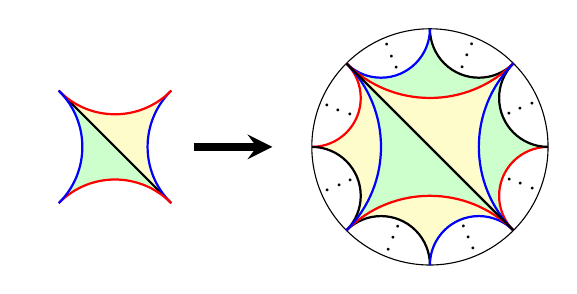
\begin{tikzpicture}
    \begin{scope}[shift={(0.50,-0.0)},rotate=-45]
      \clip (0,0) circle (1.01);
      \fill[yellow!20!white]
         (180:1.00) arc(270:360:1.00)
                    arc(180:270:1.00)
         -- cycle;
      \fill[green!20!white]
         (180:1.00) arc( 90:  0:1.00)
                    arc(180: 90:1.00)
         -- cycle;

      \draw[thick, black] (180:0.75*1.4142) -- (  0:0.75*1.4142);
      \draw[thick, blue ] ( 45:1.00*1.4142) circle (1.00);
      \draw[thick, red  ] (315:1.00*1.4142) circle (1.00);
      \draw[thick, red  ] (135:1.00*1.4142) circle (1.00);
      \draw[thick, blue ] (225:1.00*1.4142) circle (1.00);
    \end{scope}

    \draw[line width=1mm, ->, >={stealth}] (1.5, 0.0) -- (2.5,0);

    \begin{scope}[shift={(4.5,0)}]
      \draw (0,0) circle (1.5);
      %\clip (0,0) circle (1.51);
      %\fill[even odd rule]
      %\fill[yellow!20!white] (0,0) circle (1.5);

      \fill[yellow!20!white]
            (315:1.5) arc( 45:180:1.5*0.41421)
                      arc(  0:135:1.5*0.41421)
                      arc(315:450:1.5*0.41421)
                      arc(270:405:1.5*0.41421)
                      arc(225:360:1.5*0.41421)
                      arc(180:315:1.5*0.41421)
                      arc(135:270:1.5*0.41421)
                      arc( 90:225:1.5*0.41421)
        ;

      \fill[thick, even odd rule, fill=green!20!white]
            (315:1.5) arc(225: 90:1.5*0.41421)
                      arc(270:135:1.5*0.41421)
                      arc(315:180:1.5*0.41421)
                      arc(360:225:1.5*0.41421)
                      arc(225:315:1.5        )
                      arc(135:225:1.5        )
                      to (135:1.5)
                      arc(405:315:1.5        )
                      arc(135: 45:1.5        )
        ;

        \draw[thick, red  ]   (315:1.5) arc(225: 90:1.5*0.41421);
        \draw[thick, black]   (  0:1.5) arc(270:135:1.5*0.41421);
        \draw[thick, black]   ( 45:1.5) arc(315:180:1.5*0.41421);
        \draw[thick, blue ]   ( 90:1.5) arc(360:225:1.5*0.41421);
        \draw[thick, red  ]   (135:1.5) arc(405:270:1.5*0.41421);
        \draw[thick, black]   (180:1.5) arc(450:315:1.5*0.41421);
        \draw[thick, black]   (225:1.5) arc(135:  0:1.5*0.41421);
        \draw[thick, blue ]   (270:1.5) arc(180: 45:1.5*0.41421);

        \draw[thick, red  ] (315:1.5) arc( 45:135:1.5);
        \draw[thick, blue ] (225:1.5) arc(315:405:1.5);
        \draw[thick, red  ] (135:1.5) arc(225:315:1.5);
        \draw[thick, blue ] ( 45:1.5) arc(135:225:1.5);

        \draw[thick, black] (315:1.5) -- (135:1.5);

        \node at (0*45 + 22.5:1.25) {\rotatebox{ 22.5}{$\cdots$}};
        \node at (1*45 + 22.5:1.25) {\rotatebox{ 67.5}{$\cdots$}};
        \node at (2*45 + 22.5:1.25) {\rotatebox{112.5}{$\cdots$}};
        \node at (3*45 + 22.5:1.25) {\rotatebox{157.5}{$\cdots$}};
        \node at (4*45 + 22.5:1.25) {\rotatebox{202.5}{$\cdots$}};
        \node at (5*45 + 22.5:1.25) {\rotatebox{247.5}{$\cdots$}};
        \node at (6*45 + 22.5:1.25) {\rotatebox{292.5}{$\cdots$}};
        \node at (7*45 + 22.5:1.25) {\rotatebox{337.5}{$\cdots$}};
    \end{scope}
  \end{tikzpicture}
\end{document}
